\section{Remplacer les éclairages d'un scooter}

Louise doit remplacer un des deux feux arrière de son scooter. Elle trouve deux modèles de lampes : une de tension nominale 12 V et une autre de tension nominale 12 V. Le circuit de son scooter est alimenté par une batterie de 12 V sur laquelle est également branchée la lampe du phare avant.


	\begin{center}
		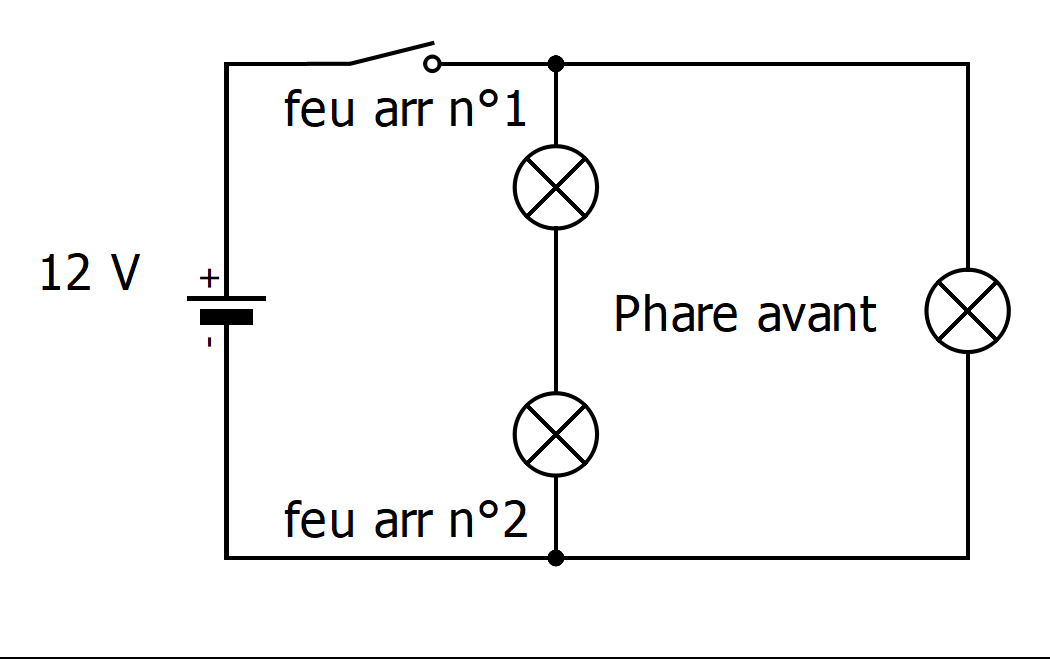
\includegraphics[scale=0.45]{scoot}
	\end{center}


\begin{questions}
	\question Quelle est la valeur de la tension aux bornes du phare avant ?
	
	\question Quelle est la valeur de la tension aux bornes de l'ensemble des deux feux arrière ?
		
	\question Calculer la tension aux bornes de chaque feu arrière (les lampes sont identiques).
	
	
	\question Indiquer le modèle de lampe que Louise doit choisir.
	
\end{questions}
%\ \label{LastPage}

\end{document}